\documentclass{article}
\usepackage{amsmath}
\usepackage{tikz}
\usetikzlibrary{calc,decorations.markings,decorations.pathmorphing,arrows.meta}
% set up externalization
\usetikzlibrary{external}
\tikzset{external/system call={latex \tikzexternalcheckshellescape -halt-on-error
-interaction=batchmode -jobname "\image" "\texsource";
dvips -o "\image".ps "\image".dvi;
ps2eps "\image.ps"}}
\tikzexternalize
\begin{document}
%---------------------------------------------------------------------------------
%
\input{./tikz_figures/fundamental_res.tex}
%
%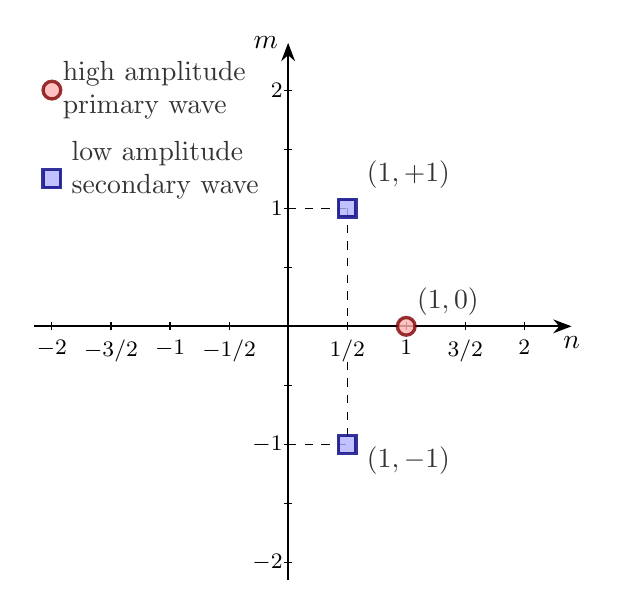
\begin{tikzpicture}[>=Stealth,scale=0.75]
  % Configurable parameters
  \def\pointwidth{0.15}                     % Half Width/radius of plotted points
  \newcommand{\axlables}{\normalsize}       % Axis label font size
  \newcommand{\annotations}{\normalsize}    % Annotations font size
  \newcommand{\ticklables}{\footnotesize}   % tick label font size
  %
  % Grid (uncomment below if necessary)
  %\draw[step=1.0cm,gray,dotted,thin] (-4.9,-4.9) grid (4.9,4.9);
  %
  % Axes
  \draw[thick,->] (-4.3,0) -- (4.8,0)
    node[below] {\axlables$n$};
  \draw[thick,->] (0,-4.3) -- (0,4.8)
    node[left] {\axlables$m$};
  %
  % Tick labels
  \draw (-4,2pt)--(-4,-2pt) node[below]      {\ticklables$-2$};
  \draw (-3,2pt)--(-3,-2pt) node[below]      {\ticklables$-3/2$};
  \draw (-2,2pt)--(-2,-2pt) node[below]      {\ticklables$-1$};
  \draw (-1,2pt)--(-1,-2pt) node[below]      {\ticklables$-1/2$};
  \draw (1,2pt)--(1,-2pt)   node[below]      {\ticklables$1/2$};
  \draw (2,2pt)--(2,-2pt)   node[below]      {\ticklables$1$};
  \draw (3,2pt)--(3,-2pt)   node[below]      {\ticklables$3/2$};
  \draw (4,2pt)--(4,-2pt)   node[below]      {\ticklables$2$};
  %
  \draw (-2pt,-4) -- (2pt,-4)  node[left]  {\ticklables$-2$};
  \draw (-2pt,-3) -- (2pt,-3);
  \draw (-2pt,-2) -- (2pt,-2)  node[left]  {\ticklables$-1$};
  \draw (-2pt,-1) -- (2pt,-1);
  \draw (-2pt,1) -- (2pt,1);
  \draw (-2pt,2)  -- (2pt,2)   node[left]  {\ticklables$1$};
  \draw (-2pt,3) -- (2pt,3);
  \draw (-2pt,4)  -- (2pt,4)   node[left]  {\ticklables$2$};
  %
  % Connecting lines
  \draw[dashed] (0,2) -- (1,2);
  \draw[dashed] (0,-2) -- (1,-2);
  \draw[dashed] (1,2) -- (1,0);
  \draw[dashed] (1,-0.6) -- (1,-2);
  %
  % Annotations
  \filldraw[fill=red!30!white,opacity=0.8,draw=red!50!black,very thick] 
    (2,0) circle [radius=\pointwidth]
    node[above right] {\annotations$(1,0)$};
  \filldraw[fill=blue!30!white,opacity=0.8,draw=blue!50!black,very thick] 
    (1-\pointwidth,-2-\pointwidth) rectangle (1+\pointwidth,-2+\pointwidth) 
    node[below right] {\annotations$(1,-1)$};
  \filldraw[fill=blue!30!white,opacity=0.8,draw=blue!50!black,very thick] 
    (1-\pointwidth,2-\pointwidth) rectangle (1+\pointwidth,2+\pointwidth) 
    node[above right] {\annotations$(1,+1)$};
  \filldraw[fill=red!30!white,opacity=0.8,draw=red!50!black,very thick] 
    (-4,4) circle [radius=\pointwidth]
    node[right,text width=2.5cm] {\annotations high amplitude primary wave};
  \filldraw[fill=blue!30!white,opacity=0.8,draw=blue!50!black,very thick] 
    (-4-\pointwidth,2.5-\pointwidth) rectangle (-4+\pointwidth,2.5+\pointwidth) 
    node[right,text width=2.5cm] {\annotations low amplitude secondary wave};
  %
\end{tikzpicture}
%
%\input{./tikz_figures/oblique_res.tex}
%
%---------------------------------------------------------------------------------
\end{document}